\documentclass[11pt]{article}

\usepackage[a4paper]{geometry}

\usepackage[T1]{fontenc}

\usepackage[ngerman]{babel}
\babelprovide[hyphenrules=ngerman-x-latest]{ngerman} % dehyph-exptl

\usepackage{caption}
\usepackage{subcaption}
\usepackage{graphicx}
\graphicspath{{images/}}

\usepackage{float}

\usepackage[all]{nowidow}

\usepackage[svgnames]{xcolor}

\usepackage[backend=biber,style=numeric-comp]{biblatex}
\addbibresource{survey-paper.bib}

\usepackage[german=quotes]{csquotes}
\SetCiteCommand{\autocite}

\usepackage{listings}

\lstset{
  basicstyle=\ttfamily,
}

\newcommand{\thetitle}{Survey: Service Discovery in der Smart City}
\newcommand{\theauthors}{Tristan Damm, Ellen Landschoof, Lukas Obermann, Louis Richter, Tjorben Wade}
\newcommand{\thesubject}{Forschungsprojekt, Master Angewandte Informatik, Sommersemester 2022, Hochschule Flensburg}

\usepackage{hyperref}
\hypersetup{
  pdftitle={\thetitle{}},
  pdfauthor={\theauthors{}},
  pdfsubject={\thesubject{}},
  pdfkeywords={},
  hidelinks,
  pdfpagemode=UseOutlines,
  pdfdirection={L2R},
  pdfduplex=Simplex,
  pdfpagelayout=TwoPageRight,
}

\usepackage{bookmark}
\bookmarksetup{numbered,open}

\usepackage[skip=2mm, indent=0pt]{parskip}

\usepackage{multicol}

\usepackage[nonumberlist,automake]{glossaries-extra}
\makeglossaries{}
\setabbreviationstyle{short-nolong}
\setabbreviationstyle[acronym]{long-short}
\setglossarystyle{list}
\loadglsentries{glossary}

\title{\thetitle{}}
\author{\theauthors{}}

\begin{document}

\pagenumbering{gobble}
\maketitle

\pdfbookmark[chapter]{\contentsname}{toc}
\newpage

\tableofcontents
\newpage
\pagenumbering{arabic}

% \section{Einleitung}

% Dies ist eine Einleitung.

% \begin{itemize}
%   \item List item
%   \item Test
% \end{itemize}

% \begin{enumerate}
%   \item test
% \end{enumerate}

% \enquote{Dies ist ein Zitat.} \autocites[vgl.][]{Apple.HIG}{Apple.HIG}.

% \autocite[vgl.][]{GermanConventionBureau.2021.DKaSbViDvunCpB}

% \textcquote[vgl.][]{Apple.HIG}{Individualisten, mit dem Ziel der persönlichen Einkommens- und Lebenslustmaximierung}

% \subsection{Sub }

% \subsubsection{Sub}

\addcontentsline{toc}{section}{Abstract}
\section*{Abstract}\label{sec:abstract}

Die \gls{sd} in der Smart City beschreibt ein Verfahren, womit \glsxtrshort{iot}-Systeme in der Stadt öffentlich dem Bürger zugänglich gemacht werden.
Um dieses Verfahren zu ermöglichen, gibt es verschiedene \glsxtrshort{sd}-Ansätze, wovon drei (Semantisch, Kontextabhängig und Quality-of-Service-basiert) genauer betrachtet werden.
Diese Verfahren beschreiben aber eine abstrakte Definition und keinen vordefinierten Standard.
Somit sind diese eher ungeeignet oder mit sehr viel Aufwand verbunden, um eine \gls{sd} in der Smart City zu realisieren.
Webstandards, wie das von der W3C definierte \gls{wot}, beschreibt bereits eine genaue Architektur für eine \gls{sd}.
Mithilfe von \glspl{td} werden Metadaten mit \glspl{thing} verknüpft, welche dann von einem Service zur Verfügung gestellt werden.
Die Punkte Sicherheit und Datenschutz spielen dabei auch eine Rolle, werden aber nicht genauer betrachtet, da sie für eine öffentliche \gls{sd} nur teilweise relevant sind.
Das \gls{wot} liefert, auch wenn die Spezifikation noch nicht vollständig ist, ein genaues Verfahren, womit eine \gls{sd} in der Smart City realisiert werden kann.
Es bestehen aber immer noch Probleme bei der Definition von Ontologien und von \gls{qos}[-Aspekten] für die \gls{sd}.

\section{Einleitung}\label{sec:introduction}

Über die letzten Jahre haben viele Städte damit begonnen, unterschiedliche Sensoren zu verbauen.
Diese werden unter anderem dazu genutzt, um zu prüfen, ob ein Parkplatz frei ist, wie gut oder schlecht die Luftqualität ist oder wie warm es aktuell ist \autocite{Chaudhari.2020.LTEACRaDC}.
Darüber hinaus können viele weitere Werte gemessen werden.

Bei den so entstandenen Netzen handelt es sich zumeist um sogenannte \gls{lpwan}[s]. Diese können auf Basis unterschiedlicher Technologien aufgebaut sein und funktionieren daher nicht alle einheitlich. Das hat zur Folge, dass in den meisten Fällen nur der Ersteller des Netzes Zugriff auf die Daten hat. Eine Interaktion zwischen mehreren Netzen, um genauere Daten zu erzielen oder Daten besser verteilen zu können, wird deutlich erschwert.

Aus der Open-Data-Strategie der Bundesregierung geht hervor, dass die meisten der so gesammelten Daten von den Städten öffentlich zur Verfügung gestellt werden müssen \autocite{BMI.}.
Wie dies genau geschieht, ist den Städten selbst überlassen. Viele Daten werden unter \url{https://www.govdata.de/} zur Verfügung gestellt, aber es gibt auch andere Quellen. Zumeist müssen die Daten dabei manuell heruntergeladen werden.

Das Format der Daten unterscheidet sich ebenfalls. Während sie meisten als CSV-Datei veröffentlicht werden, sind auch PDF-, XML- und HTML-Dateien sehr häufig vertreten. Für einen großen Teil der Daten auf GovData ist zudem kein Dateityp angeben.

All das macht es schwierig, die Daten in Anwendungen einzubinden und so für den Alltag nutzbar zu machen.

Dabei helfen könnte unter anderem eine Schnittstelle, die die Daten von unterschiedlichen Sensoren für Geräte auffindbar macht.
Die größten Probleme, die sich dabei stellen, sind die Service Discovery und die verwendete Sprache, um die Sensoren zu beschreiben oder zu finden.
Dabei können Begriffe, die von Menschen leicht verknüpft werden können, von Maschinen nicht in Verbindung gebracht werden, was dazu führt, dass Services gegebenenfalls nicht gefunden werden.
Dieses zweite Problem bezieht sich daher auf die Ontologie.

In diesem Bericht werden einige Rechercheergebnisse beschrieben, die für die Arbeit in diesem Bereich von Bedeutung sind.
Dazu werden in \autoref{sec:relatedworks} zunächst verwandte Arbeiten beschrieben.
Anschließend werden in \autoref{sec:sd} einige Arten der Service Discovery dargestellt und in \autoref{sec:wot} auf das Web of Things eingegangen, bevor in \autoref{sec:discussion} die Ergebnisse diskutiert werden.
Abschließend wird in \autoref{sec:conclusion} ein Fazit gebildet.

\section{Related Works}\label{sec:relatedworks}

Es gibt zahlreiche Literatur im Bereich der \gls{sd}, in denen die verschiedene Methoden entweder allgemein oder speziell für einen bestimmten Anwendungsbereich beschrieben werden.

Die semantische \gls{sd} bietet Vorteile in der Verwendung von Ontologien \autocite{Novo.2020.SIitI} und findet auch im Bereich von \gls{wot} ihren Verwendungszweck \autocite{Serena.2018.SDitWoT}.
Es gibt aber auch einen Ansatz der in den Bereichen der Zuverlässigkeit und Sicherheit ihren Nutzen findet \autocite{Li..ADTCaQASDFftIoT}. Diese wird \gls{qos}-basierte \gls{sd} \autocite{Kosunalp.2020.SArlbQaIsdm} genannt und wurde unter anderem von \citeauthor{Kosunalp.2020.SArlbQaIsdm} behandelt.
Die Kontextabhängige \gls{sd} \autocite{Sukode.2015.CAFIIAS} arbeitet stattdessen mit den Informationen aller relevanten Entities.

Die \gls{sd} ist ein wichtiger Punkt in den \gls{iot}-Systemen und einen guten Einblick in dieses umfangreiche Themenfeld bietet die Arbeit \autocite{Achir.2022.SdasiIAsaat} von \citeauthor{Achir.2022.SdasiIAsaat}.

Für das \gls{wot} existiert ein sehr aktuelles und umfassendes Paper von \citeauthor{Sciullo.2022.ASotWoT}, welches auf alle Ansätze der letzten Jahrzehnte eingeht und in diversen Kategorien systematisch analysiert und vergleicht \autocite{Sciullo.2022.ASotWoT}. Auf der Webseite des \gls{w3c} finden sich verschiedene Spezifikationen und Richtlinien zum Thema \gls{wot} \autocites{w3c.wot.architecture.20200408}{w3c.wot.td.20200623}{w3c.wot.discovery.20210602}{w3c.wot.spg.20191106}.

In dieser Arbeit werden die für uns relevantesten Verfahren kurz beschrieben, was als eine Recherchearbeit für ein Projekt im Bereich der \glsxtrshort{iot}-Discovery dient.

\section{Service Discovery}\label{sec:sd}

Das \gls{iot} hat heutzutage einen großen Einfluss auf unseren Alltag.
Über eine Vielzahl von Sensoren werden dabei eine Menge an Daten aufgezeichnet, die anschließend in den unterschiedlichsten Services zur Verfügung gestellt werden.
Dabei ist das Auffinden und Auswählen des richtigen Services nicht immer ganz einfach.
Es haben sich daher unterschiedliche Arten der \gls{sd} entwickelt, die jeweils für unterschiedliche Bereiche besonders gut geeignet sind \autocite{Achir.2020.AtosdaiI}.

Im folgenden Abschnitt werden drei Arten der \gls{sd} genauer beschrieben, die am bedeutendsten sind, wenn es darum geht, Daten aus \gls{lpwan} von Städten, wie in der Einleitung beschrieben, über eine Schnittstelle für Maschinen zugänglich zu machen.
Dabei handelt es sich um die semantische \gls{sd}, die Quality-of-Service-basierte \gls{sd} und die Kontextabhängige \gls{sd}.

\subsection{Semantisch}\label{subsec:semanticsd}

Das Ziel der semantischen \gls{sd} ist es, den Service, der am besten zu den gegebenen Ansprüchen passt, mithilfe einer Ontologie zu finden.
Eine Ontologie stellt dabei die Zusammenhänge zwischen verschiedenen Begriffen oder Eigenschaften dar, die in der Suche genutzt werden können. Die Begriffe selbst werden ebenso definiert und beschrieben, um für das jeweilige Themengebiet ein einheitliches Vokabular nutzen zu können. Auf diese Weise ist es möglich, ein gemeinsames Verständnis über ein bestimmtes Gebiet zu schaffen.
Dabei können im Gegensatz zu den meisten anderen Systemen Services nicht nur funktionale, sondern auch nicht funktionale Eigenschaften -- wie Performance, Kosten oder Zuverlässigkeit -- beachtet werden.

Zum Erstellen einer semantischen Service Discovery gibt es keine festgelegte Standardisierung, die verfolgt werden muss.
Bei bisherigen Arbeiten wurde daher jeweils ein eigener Ansatz entworfen und umgesetzt. Diese Ansätze können mehr oder weniger stark voneinander abweichen.

In der Arbeit von \citeauthor{Suraci.2008.CaSSD} \autocite{Suraci.2008.CaSSD} wird eine kontextbewusste Architektur vorgestellt, die für eine Service Discovery genutzt werden kann. Die Architektur selbst ist dabei nicht abhängig von der verwendeten Technologie und kann mit vielen vorhandenen Service-Discovery-Protokollen genutzt werden.

Im Kontrast dazu handelt die Arbeit von \citeauthor{Iqbal.12320081252008.SSDuSaS} \autocite{Iqbal.12320081252008.SSDuSaS} davon, wie Services, spezifisch mit SAWSDL und SPARQL, beschrieben werden können.
Auch \citeauthor{BenMokhtar.2006.ESSDiPCE} \autocite{BenMokhtar.2006.ESSDiPCE} bauen bei ihrer Arbeit auf spezifische Sprachen auf. Sie nutzen Amigo-S für semantische Spezifikationen und S-Ariadne, eine Erweiterung von Ariadne, als Discovery-Protokoll. Ihr Ziel war es, einen effizienten Weg zum Finden von Services zu entwickeln.

In weiteren Arbeiten geht es häufig darum, wie und auf Basis welcher Grundlagen passende Services für die Nutzer ausgewählt werden können.
\citeauthor{Majithia.2004.Rbssd} \autocite{Majithia.2004.Rbssd} haben so beispielsweise ein Framework entwickelt, dass Services basierend auf ihrem Ruf findet. Zu dem Ruf eines Services gehört dabei unter anderen dessen Zuverlässigkeit und Erreichbarkeit.
\citeauthor{Jia.2017} \autocite{Jia.2017} schlagen hingegen ein zentralisiertes, mehrstufiges semantisches Service-Matching vor, das in vier Schichten abläuft, und
\citeauthor{Zhao.2017} \autocite{Zhao.2017} legen ihren Fokus auf die Beschreibung von IoT-Services und deren Ähnlichkeit zueinander. Dabei werden die Ähnlichkeiten gemessen und ein Cluster erstellt, um ähnliche Services zu sammeln.

Ein Vorteil der semantischen Service Discovery ist, dass Ontologien mit in Betracht gezogen werden können.
Aufgrund der fehlenden Standardisierung müssen Arbeiten jedoch von Grund auf eigenständig entwickelt werden.
Das kann Vorteile mit sich bringen, aber ist gleichzeitig mit einer großen Arbeitslast verbunden und nicht für alle Projekte geeignet.

\subsection{Quality-of-Service-basiert}\label{subsec:qosbasedsd}

Bei der \glsdisp{qos}{Quality-of-Service-basierten (QoS)} \gls{sd} stehen nichtfunktionale Bewertungskriterien im Vordergrund. Diese werden auf die Sicht des Anwendenden bezogen und können als Güte für deren Anforderungen verstanden werden.

Die verschiedenen \gls{qos}-Ansätze werden für die \gls{sd} in verschiedene Unterkategorien sortiert \autocite{Achir.2020.AtosdaiI}. Je nach Optimierungsziel des Ansatzes wird dieser folgenden Kategorien zugeordnet:

\begin{itemize}
    \item Sicherheitsbasiert
    \item Energieverbrauchsbasiert
    \item Netzinfrastrukturbasiert
\end{itemize}

Des Weiteren wird eine Hybrid-Kategorie gebildet, um Ansätze, die mehrere Faktoren abdecken, aufzunehmen. Eine \gls{qos}-basierte \gls{sd} verfolgt verschiedene Ziele. Die Geschwindigkeit bei der Suche soll z.\,B.\ möglichst schnell ablaufen. Algorithmen, die sich auf dieses Ziel konzentrieren, werden daher in die Netzinfrastruktur-Kategorie eingeordnet. Andere Algorithmen, die den Prozess hinsichtlich der Sicherheit der Suche z.\,B.\ mithilfe von Authentifizierungen verbessern, können für diese Arbeit vernachlässigt werden, da es sich um einen Open-Data-Standard handeln soll. Die Kategorie für den Energieverbrauch hat, zusätzlich zur Netzinfrastruktur, eine hohe Bedeutung für den Bereich dieser Arbeit. Es muss darauf geachtet werden, dass die Services möglichst wenige und kurze Berechnungen zur \gls{sd} durchführen müssen.


Die \gls{qos}-basierte \gls{sd} nutzt unterschiedliche Verarbeitungsinformationen, basiert jedoch im Grundsatz auf vorhandenen \gls{sd}-Ansätzen, wie z.\,B.\ dem semantischen Ansatz. Das Finden der Dienste basiert häufig auf den vorhandenen Ansätzen. Nachdem ein Dienst gefunden wurde, fungiert die \glsxtrshort{qos}-basierte \gls{sd} als eine Art \glsxtrshort{qos}-Filter \autocite{Kosunalp.2020.SArlbQaIsdm}. Dadurch werden Dienste, die nicht verfügbar oder nach vorhandenen Information nicht geeignet sind, eliminiert.

SARL \autocite{Kosunalp.2020.SArlbQaIsdm} ist ein Konzept, das die \glsxtrshort{qos}-basierte \gls{sd} nutzt. Es basiert auf einem P2P-Konzept, das noch keine \glsxtrshort{qos}-Faktoren abdeckt. Die einzelnen Services kennen bei diesem Ansatz nur die Art der Daten, die sie selbst bereitstellen, und Wege zu Nachbarknoten.
Es gibt verschiedene Ansätze, den Weg zum Zielknoten (Zieldienst) zu finden.

Ein nicht \glsxtrshort{qos}-basierter Ansatz ist, die Suchanfrage ohne zusätzliche Informationen zu nutzen, von Knoten zu Knoten zu schicken, bis sie beim Ziel ankommt. Dadurch entsteht ein Nachrichtenüberfluss, der die Geschwindigkeit verlangsamt und somit für Nutzende im Hinblick auf die Zuverlässigkeit wahrnehmbar ist.

Bei einem \glsxtrshort{qos}-basierten Ansatz werden zur Weiterleitung zwischen den Knoten (Diensten) verschiedene Informationen herangezogen. Es wird ein \glsxtrshort{qos}-Ranking gebildet, das die Rückgabe eines Dienstes bestimmt. Dieses basiert auf Informationen von vorherigen Anfragen oder selbstständig gesammelten Informationen. Damit verbessert der SARL-Ansatz die \gls{qos} hinsichtlich der Netzinfrastruktur.

Die Schwierigkeit bei Verbesserungen hinsichtlich der \gls{qos} besteht darin, Mittelwege zwischen aktuellen Informationen über andere Knoten und veralteten Daten zu finden. Die Netzwerklast kann beispielsweise nicht nur von zu vielen unstrukturierten Abfragen, sondern auch von zu vielen Abfragen, die den Status einzelner Knoten erfassen, erhöht werden. Dies hat eine Verletzung der \glsxtrshort{qos}-Faktoren zur Folge.

\subsection{Kontextabhängig}\label{subsec:contextawaresd}

Dieses Kapitel beschäftigt sich mit dem Thema Kontextabhängige Service Discovery
und erklärt die verschiedenen Zusammenhänge, die damit verbunden sind. Zunächst wird jedoch der einzelne Begriff Kontext beschrieben.
Dieser wird in vielen Literaturen definiert, aber in dieser Arbeit wird der englische Begriff Kontext in dem Zusammenhang mit Kontext-Awareness verwendet und sollte nicht mit direkt mit dem deutschen Begriff Kontext verwechselt werden.

Eine sehr gute und allgemeine Definition des Begriffes Kontext lautet: \textcquote{Sukode.2015.CAFIIAS}{Context is any information
that can be used to characterize the situation of an entity. An entity is a
person, place, or object that is considered relevant to the
interaction between a user and an application, including the
user and applications themselves.}

Bezogen auf unsere Arbeit bedeutet dies, dass der Kontext jede Information ist, die zur Beschreibung einer relevanten Entität verwendet werden kann. Außerdem muss der Kontext für die \gls{sd} so strukturiert sein, dass alle beteiligten Entitäten darin zusammengefasst und verwaltet werden können.

Hier nutzt die \gls{sd} einen Kontext, welcher für jeden einzelnen Anwendungsbereich neu modelliert wird. Dafür muss im Vorfeld recherchiert werden, welche Informationen die einzelnen Entitäten liefern können und für die Interaktion wichtig sind.
Ist zum Beispiel ein Sensor in der Interaktion beteiligt, so muss die Frage geklärt werden, ob der Messwert als Information ausreicht, oder ob zusätzliche Informationen wie Hersteller, Standort, oder Größe eine wichtige Rolle spielen.

Ein weiterer wichtiger Punkt ist die Art und Weise, wie die \gls{sd} alle erforderlichen Informationen abfragen kann. Häufig besitzen die Entitäten dafür eine vordefinierte Schnittstelle, welche die bei einer Abfrage die gewünschten Werte zurückliefert.
Eine weitere Möglichkeit wäre das manuelle Eintragen von Werten. Das sollte allerdings vermieden werden, damit das System autonom bleibt. Eine mögliche Ausnahme können statische Werte sein, die sich ohnehin nicht ändern.

Haben wir ein System, das solch einen Kontext berücksichtigt, dann wird von Context-Awareness gesprochen. Es nutzt bei Anfragen eines Benutzers die vorhandenen Informationen, um eine bestmögliche Antwort zu liefern.
In dem Bereich der \gls{sd} werden so gezielt Services lokalisiert und genutzt.


\section{\Glsfmtlong{wot}}\label{sec:wot}

Ein Problem bei der Service Discovery im \gls{iot} sind immer die Interoperabilität und Kompatibilität zwischen verschiedenen Systemen. Ein Bereich, in dem diese Aspekte von großer Relevanz sind, ist das Internet. Webtechnologien müssen für eine Vielzahl von Geräten und Anwendungen funktionieren. So wurde das Internet auch als Inspirationsquelle für die Lösung solcher und anderer Probleme im \gls{iot} genutzt. Diese Kombination wird im Allgemeinen als \gls{wot} bezeichnet.

Das \gls{wot} ist eine Erweiterung des \gls{iot}, die grundsätzlich die \glspl{thing} (oder deren \glspl{intermediary}) um eine Web-Server-Komponente erweitert, mit der Kommunikation von außen über einen \gls{uri} oder \gls{iri} initialisiert und durchgeführt werden kann.

Im Laufe der Jahre haben sich dabei die \glsxtrshort{wot}-Spezifikationen und -Empfehlungen des \gls{w3c}[s], welches auch die Spezifikationen für andere Webtechnologien herausbringt, zu den meistgenutzten und vollständigsten entwickelt \autocite[vgl.][47573]{Sciullo.2022.ASotWoT}, weshalb diese in den nachfolgenden Unterkapiteln näher betrachtet werden.

Es gibt verschiedene Spezifikations- und Richtliniendokumente, die das \gls{w3c} bereitstellt.

\begin{itemize}
  \item Die \emph{Architecture} \autocite{w3c.wot.architecture.20200408} gibt einen Überblick über das \gls{wot}, welches vom \gls{w3c} standardisiert bzw.\ empfohlen wird.
  \item Die \emph{\glsfmtlong{td}} \autocite{w3c.wot.td.20200623} ist die Spezifikation für das Format, in dem einzelne \glspl{wt} beschrieben werden.
  \item Die \emph{Binding Templates} \autocite{w3c.wot.bt.20200130} sind Richtlinien, wie Netzwerkschnittstellen definiert werden sollen.
  \item Die \emph{Scripting API} \autocite{w3c.wot.scriptingapi.20201124} beschreibt eine (optionale) JavaScript-API, die für eine Anwendung genutzt werden kann, die auf das \gls{wot} zugreifen können soll.
  \item Die \emph{Discovery} \autocite{w3c.wot.discovery.20210602} beschreibt, wie sich sowohl \glspl{thing} nach außen bekannt machen können, als auch Anwendungen nach existierenden \glspl{thing} erkundigen können. Zum Zeitpunkt der Erstellung dieses Berichts ist dieses Dokument jedoch noch nicht in einem fertigen Zustand gewesen.
  \item Die \emph{Security und Privacy Guidelines} \autocite{w3c.wot.spg.20191106} enthalten Richtlinien zur sicheren Implementierung und Konfiguration von \glspl{thing} sowie möglicherweise auftretende Probleme und deren Behebung.
\end{itemize}

Es gibt noch weitere Dokumente, die jedoch nicht relevant für den Anwendungszweck der Service Discovery sind und daher hier nicht angeführt werden. Sie können unter \url{https://www.w3.org/TR/?tag=wot} eingesehen werden.

\subsection{Architekturüberblick}\label{subsec:wotarchitecture}

Für das \gls{wot} gibt es verschiedenste Anwendungsfälle. All diese haben Gemeinsamkeiten und Unterschiede, aus denen sich die Anforderungen an eine \glsxtrshort{wot}-Architektur \autocite[vgl.][]{w3c.wot.architecture.20200408} ergeben.

\begin{figure}[H]
  \centering
  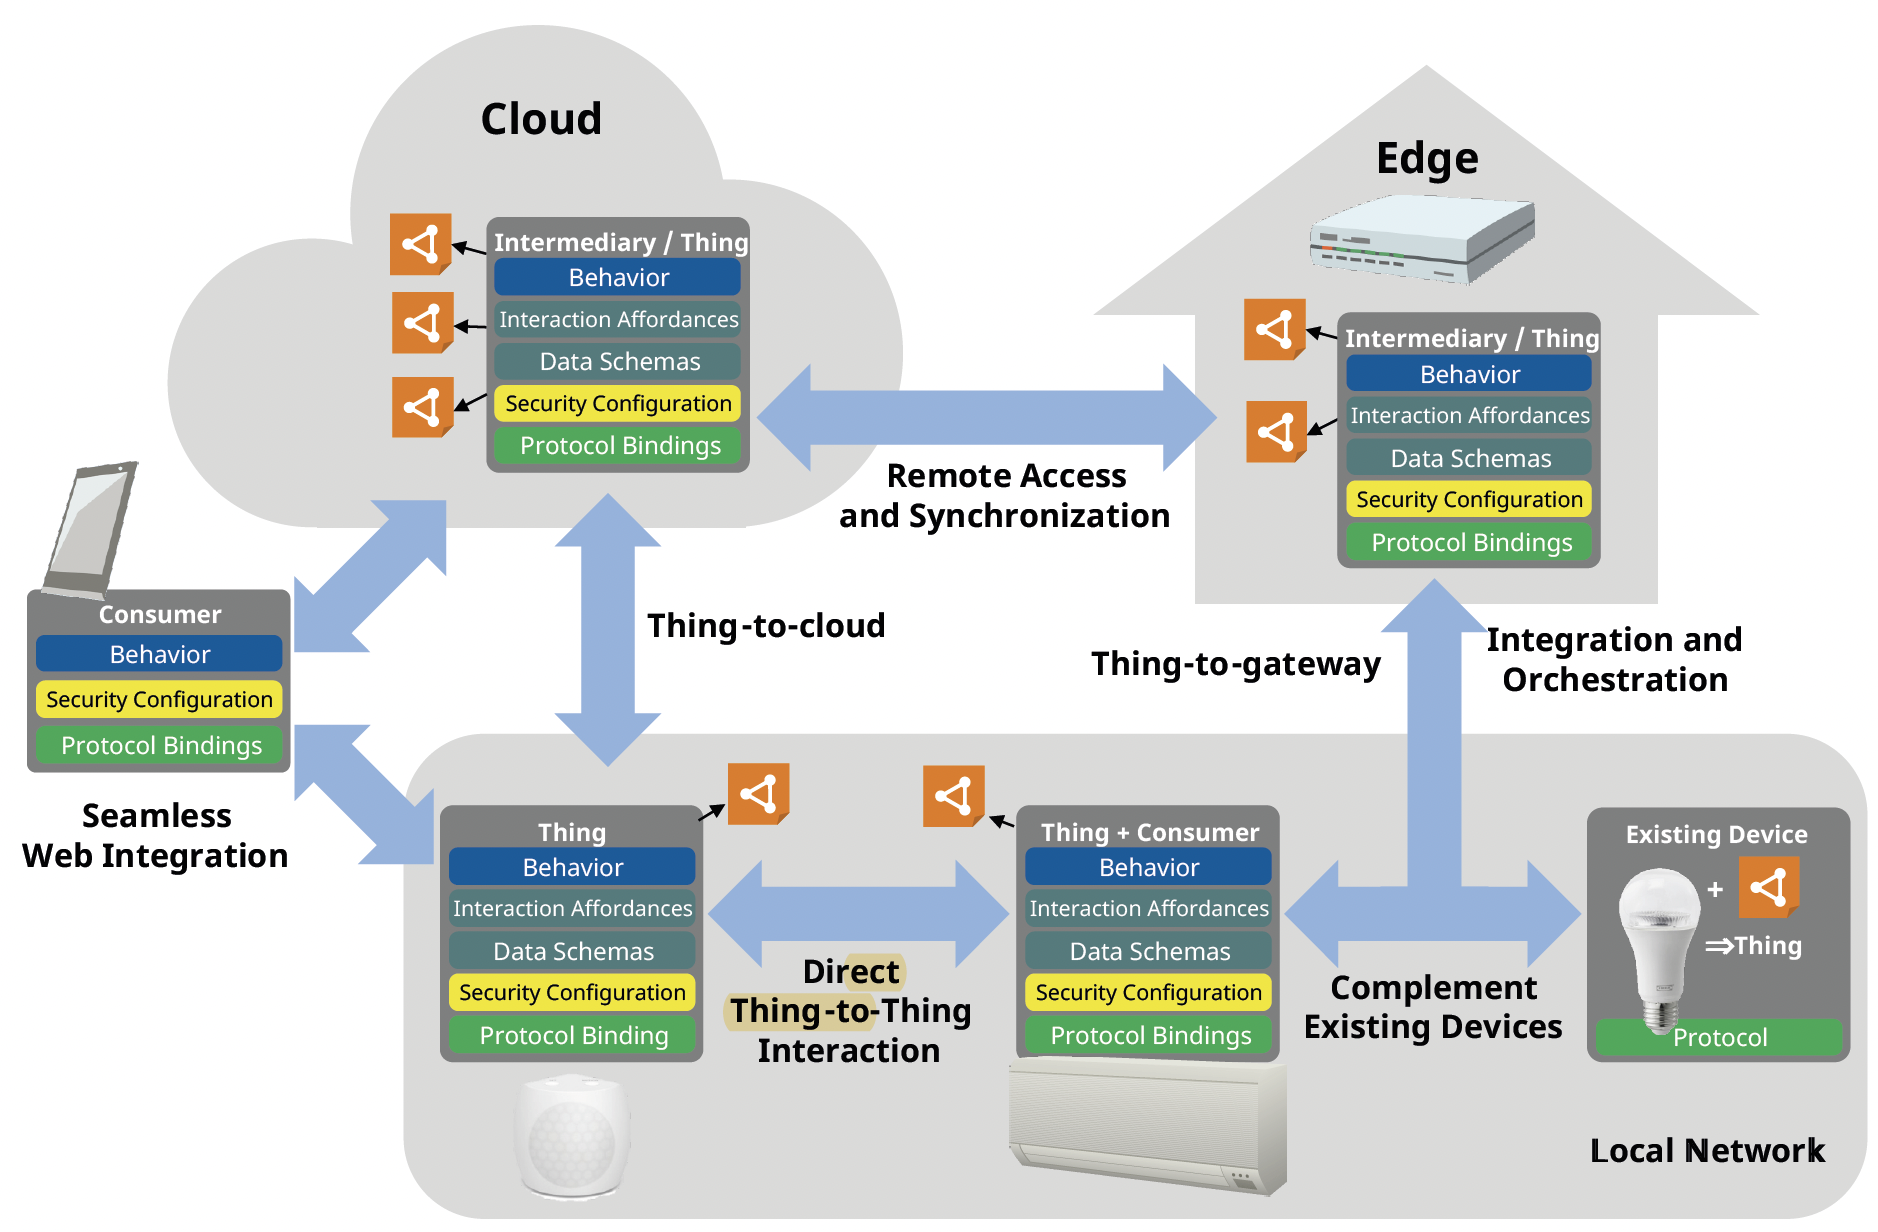
\includegraphics[width=12cm]{abstract-architecture-overview.png}
  \caption{\glsxtrshort{wot}-Architektur}\label{fig:wot_abstract_architecture}
\end{figure}

% Problem Heterogenität

Durch die starke Heterogenität der Anwendungen und Geräte, aber auch der bereits existierenden \glsxtrshort{iot}-Systeme, entsteht eine Vielzahl von Anforderungen. Diese lassen sich häufig in zwei Kategorien einteilen: Positive Anforderungen, die in allen betroffenen Entitäten umgesetzt werden können, oder negative Anforderungen, die nicht in allen betroffenen Entitäten umgesetzt werden können und wodurch die Anforderung aus einer Unabhängigkeit von diesem Teilaspekt besteht. Im Zentrum stehen vier Kernelemente: Flexibilität, Kompatibilität, Skalierbarkeit und Interoperabilität.

% Hardware

Die Architektur muss demnach hardwareunabhängig sein. Auch bestimmte Technologien können nicht vorausgesetzt werden, denn es muss Kompatibilität zu allen vorhandenen Geräten und Systemumgebungen sichergestellt werden. Dadurch fokussiert sich das \gls{wot} des \gls{w3c}[s] auf höhere Systemebenen und somit vor allem die Kommunikationsebene.

% Web Thing

Auf dieser Basis wird die Architektur eines \gls{wt}[s] in verschiedene Bereiche unterteilt. Neben dem eigentlichen \emph{Verhalten} sind das \emph{Interaktionsaffordanzen}, die dazugehörigen \emph{Datenschemata}, die \emph{Sicherheitskonfiguration} und \emph{Protokollbindungen}. Dabei sind die Protokollbindungen die Definition, wie konkret Interaktionen durchgeführt werden können, während die Affordanzen nur beschreiben, was möglich ist, unabhängig von Protokollen oder Datenkodierung. Das \emph{Interaktionsmodell} beschreibt dabei neben Navigation drei weitere Typen von Interaktionsaffordanzen:

\begin{itemize}
  \item \emph{Eigenschaften} bilden den Zustand eines \gls{thing}[s] ab.
  \item Mittels \emph{Aktionen} kann der Zustand eines \gls{thing}[s] oder eine Funktion auf diesem geändert bzw.\ aufgerufen werden. % TODO: Aktionen
  \item \emph{Ereignisse} finden bei Zustandsänderungen statt und können Daten asynchron an \gls{consumer} senden.
\end{itemize}

Dabei werden die einzelnen Interaktionsschnittstellen durch Verknüpfungen in Form von \gls{uri}[s] und optionale Zusatzbeschreibungen maschinenlesbar definiert.

\begin{figure}[H]
  \centering
  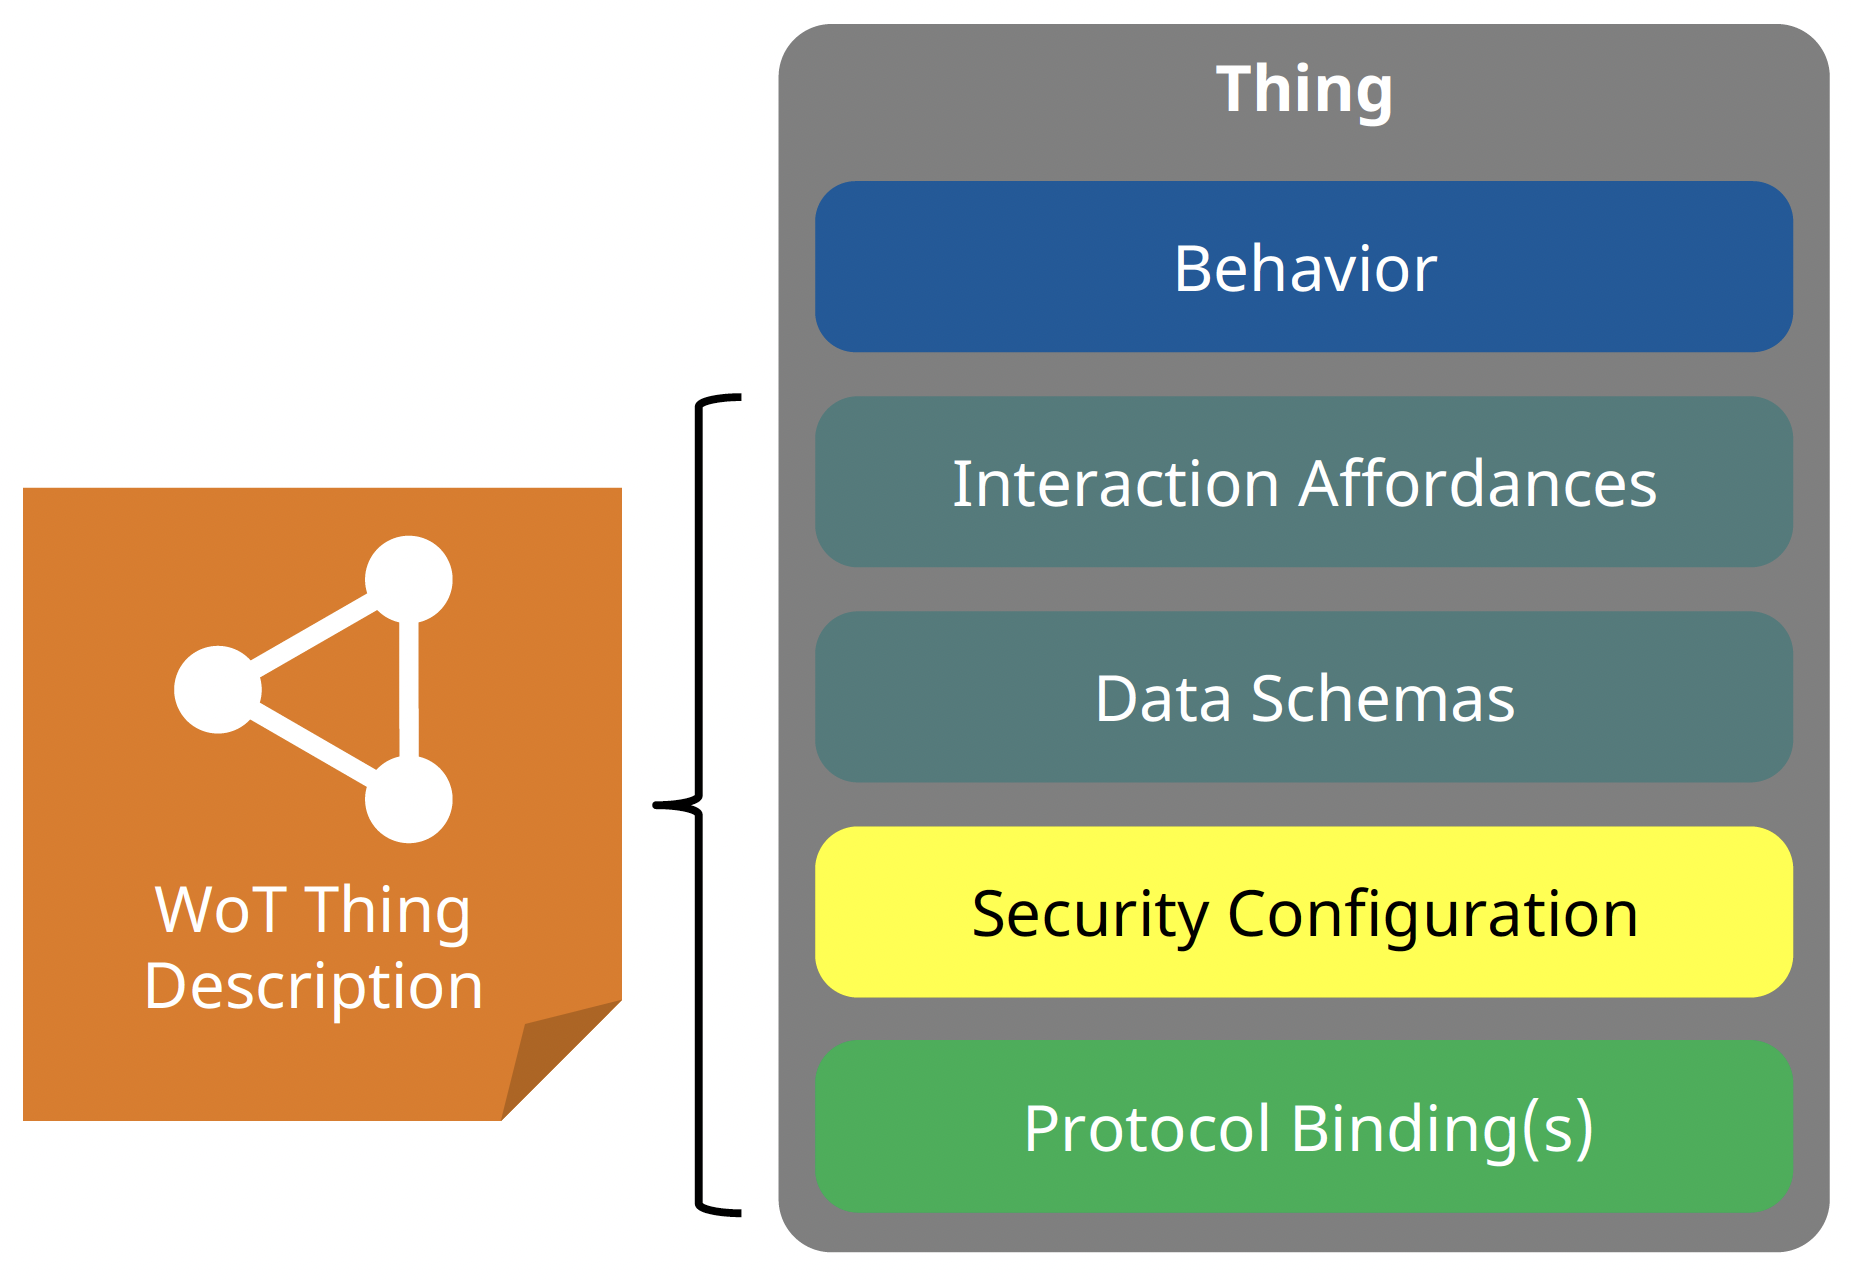
\includegraphics[width=8cm]{thing-architecture.png}
  \caption{\gls{thing}-Architektur}\label{fig:td_thing_architecture}
\end{figure}

% Thing-Beschreibung

Jedes \gls{thing} (oder dessen \gls{intermediary}) muss diese Funktionalitäten und Metadaten über sich bereitstellen können. Dazu gehören die bereits erwähnten Interaktionsaffordanzen, Datenschemata, die Sicherheitskonfiguration und die Protokollbindungen, neben dem Namen oder der Version des \gls{thing}[s] aber nicht zuletzt auch verwandte \glspl{thing}. Diese Eigenschaften sollen sowohl menschenlesbar als auch maschinenlesbar sein, semantisch annotiert werden sowie, falls zutreffend, Internationalisierung unterstützen können. Die Beschreibung dieser Eigenschaften wird \gls{td} genannt. Die \gls{td} wird als \gls{json} übermittelt und dient als Einstiegspunkt für ein \gls{thing}.

Im Idealfall wird eine \gls{td} direkt auf dem jeweiligen \gls{thing} erstellt und bereitgestellt. Domänenspezifisches Vokabular wird dabei zwar nicht durch die \glsxtrshort{wot}-Spezifikationen des \gls{w3c} abgedeckt, da die \gls{td} aber \gls{jsonld} implementiert, kann beliebiges Vokabular als Kontext eingebunden werden. Eine genauere Beschreibung der \glsfmtlong{td} ist in \autoref{subsec:wottd} zu finden.

% Protokolle

\Glspl{wt} müssen verschiedene Protokolle unterstützen können. Dazu zählen nicht nur Internetprotokolle, sondern auch Protokolle, die im \gls{lan} genutzt werden. Außerdem sollten auch Kombinationen von Protokollen genutzt werden können. So soll grundsätzlich mit \glsxtrshort{rest}-\glsxtrshortpl{api} gearbeitet werden, jedoch soll auch der Datenaustausch mit dem \gls{pubsub}-Muster möglich sein.

% Discovery

Damit mit einem \gls{wt} -- also der Repräsentation eines \gls{thing}[s] im Web -- interagiert werden kann, muss ein \gls{consumer} aber von diesem wissen. Dafür muss nach dem \gls{wt} gesucht werden können. Diese Suche muss syntaktisch (Attribute, …) und semantisch (Funktionalitäten auf Basis eines einheitlichen Vokabulars) über verschiedene Formate möglich sein. Es kann hilfreich sein, für die Erkundung ein Verzeichnis zu nutzen, bei dem sich die einzelnen \glspl{wt} automatisiert oder manuell registrieren können und welches darauf basierende Suchanfragen bearbeiten kann. (Siehe dazu auch \autoref{subsec:wotdiscovery}.)

% Sicherheit

Die \gls{td} umfasst auch Angaben zur Sicherheit nach außen. Dazu gehören z.\,B.\ Authentifizierungsmethoden wie Basic oder OAuth2.0. Grundsätzlich sollten (laut der Spezifikation) \gls{td}[s] nur autorisierten Personen zugänglich gemacht werden, da die enthaltenen Metadaten potenziell sensible Informationen beinhalten können. Trotzdem -- oder gerade deswegen -- sollten die Personen, die \gls{td}[s] erstellen oder verwalten, darauf achten, dass nur öffentliche Sicherheitsinformationen -- wie die jeweilige Authentifizierungsmethode -- in einer \gls{td} vorkommen.

% Barrierefreiheit

Barrierefreiheit ist im Rahmen der Spezifikationen kein Thema, da es um die Kommunikation zwischen Anwendungen und Geräten geht und Personen nicht direkt auf das \gls{wot} zugreifen. Allerdings gilt es zu bedenken, dass mit entsprechenden Annotationen möglicherweise Code oder ganze Interfaces generiert werden könnten, sodass die Integration von Barrierefreiheit durchaus auch Auswirkungen auf andere Bereiche hätte.

Weitere Anforderungen, die jedoch nicht zur Thematik der Service Discovery beitragen, können in \citetitle{w3c.wot.architecture.20200408} \autocite{w3c.wot.architecture.20200408} nachgelesen werden.

\subsection{\Glsfmtlong{td}}\label{subsec:wottd}

Die \glsfirst{td} \autocite{w3c.wot.td.20200623} hat, wie in \autoref{subsec:wotarchitecture} bereits oberflächlich beschrieben, vier Hauptbestandteile:

\begin{itemize}
  \item Beschreibende Metadaten über das \gls{thing};
  \item Interaktionsaffordanzen, die beschreiben, wie man das \gls{thing} nutzen kann;
  \item Schemata, die beschreiben, wie die Daten aussehen (müssen), die entweder an das oder von dem \gls{thing} geschickt werden;
  \item Verweise auf verwandte \glspl{thing} oder Dokumente.
\end{itemize}

Eine \gls{td} wird in \glsxtrshort{json} verfasst und folgt dem \glsxtrshort{jsonld}-Standard. Dabei existieren verschiedene Vokabulare für die unterschiedlichen Bereiche des Informationsmodells, die als Kontext verwendet werden können.

Jedes Vokabular enthält im Grunde Definitionen von Datenstrukturen, die im objektorientierten Kontext als Objekte verstanden werden können. Das Kernvokabular definiert dabei den grundsätzlichen Aufbau einer \gls{td}, während es dabei die anderen spezifischeren Vokabulare für ihre jeweiligen Teilbereiche referenziert.

\subsubsection{Kernvokabular}

Das Kernvokabular deckt das Interaktionsmodell aus Eigenschafts-, Aktions- und Ereignisinteraktionsaffordanzen ab.

\begin{figure}[H]
  \centering
  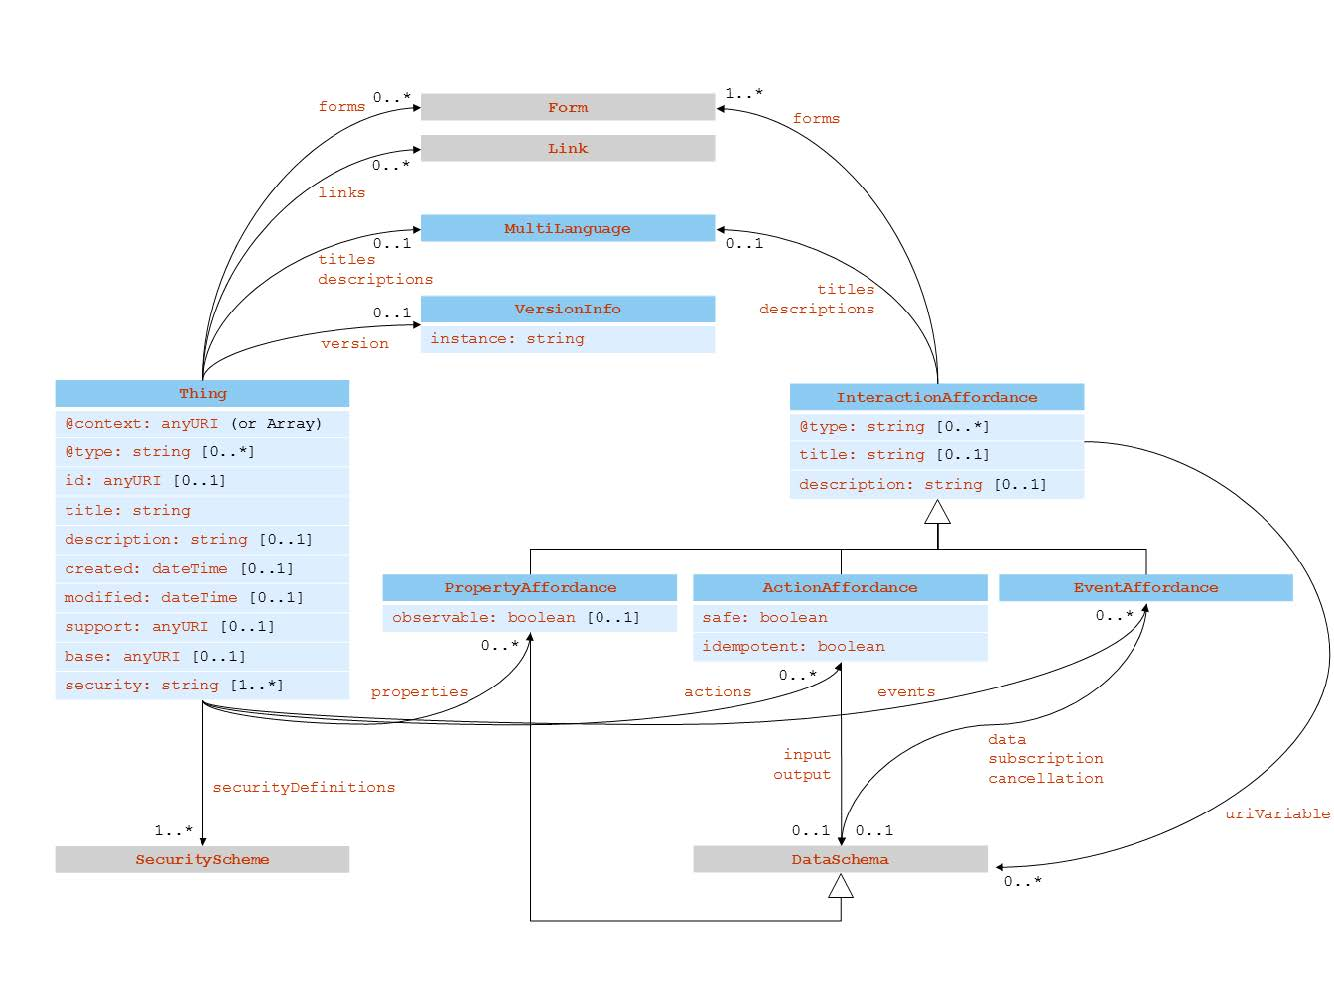
\includegraphics[width=\textwidth]{td-core-vocabulary.jpg}
  \caption{\glsxtrshort{td} Kernvokabular}\label{fig:td_core_vocabulary}
\end{figure}

Das \lstinline{Thing} ist dabei das Grundobjekt, welches die Wurzel eines \glsxtrshort{td}-Dokuments definiert. Dazu gehören der \gls{uri} des \gls{thing}[s], \glsxtrshort{jsonld}-Annotationen, Beschriftungen, Metadaten, vor allem aber die einzelnen Bereiche des Interaktionsmodells, Links zu anderen \glspl{thing}, Hypermediakontrolldefinitionen sowie Sicherheitsmechanismen des \gls{thing}[s].

Es gibt drei Arten von \lstinline{InteractionAffordance}s:

\begin{itemize}
  \item \lstinline{PropertyAffordance}s
  \item \lstinline{ActionAffordance}s
  \item \lstinline{EventAffordance}s
\end{itemize}

Allen ist gemein, dass sie Beschriftungen haben, Hypermediakontrollen, die beschreiben, wie mit ihnen interagiert werden kann, sowie Schemata für Werte, die übergeben werden müssen. Für eine \lstinline{PropertyAffordance} kann zusätzlich definiert werden, ob diese überwacht werden kann. Bei einer \lstinline{ActionAffordance} kann noch definiert werden, wie Eingabe- und Ausgabedaten aussehen sollen und wie sich die Aktion verhält. Bei einer \lstinline{EventAffordance} können stattdessen die Daten definiert werden, die bei der Abonnierung und Deabonnierung benötigt werden sowie die, die dann erhalten werden.

\subsubsection{Datenschemavokabular}

Das Datenschemavokabular leitet sich aus der JSON-Schema-Spezifikation \autocite{jsonschema} ab.

\begin{figure}[H]
  \centering
  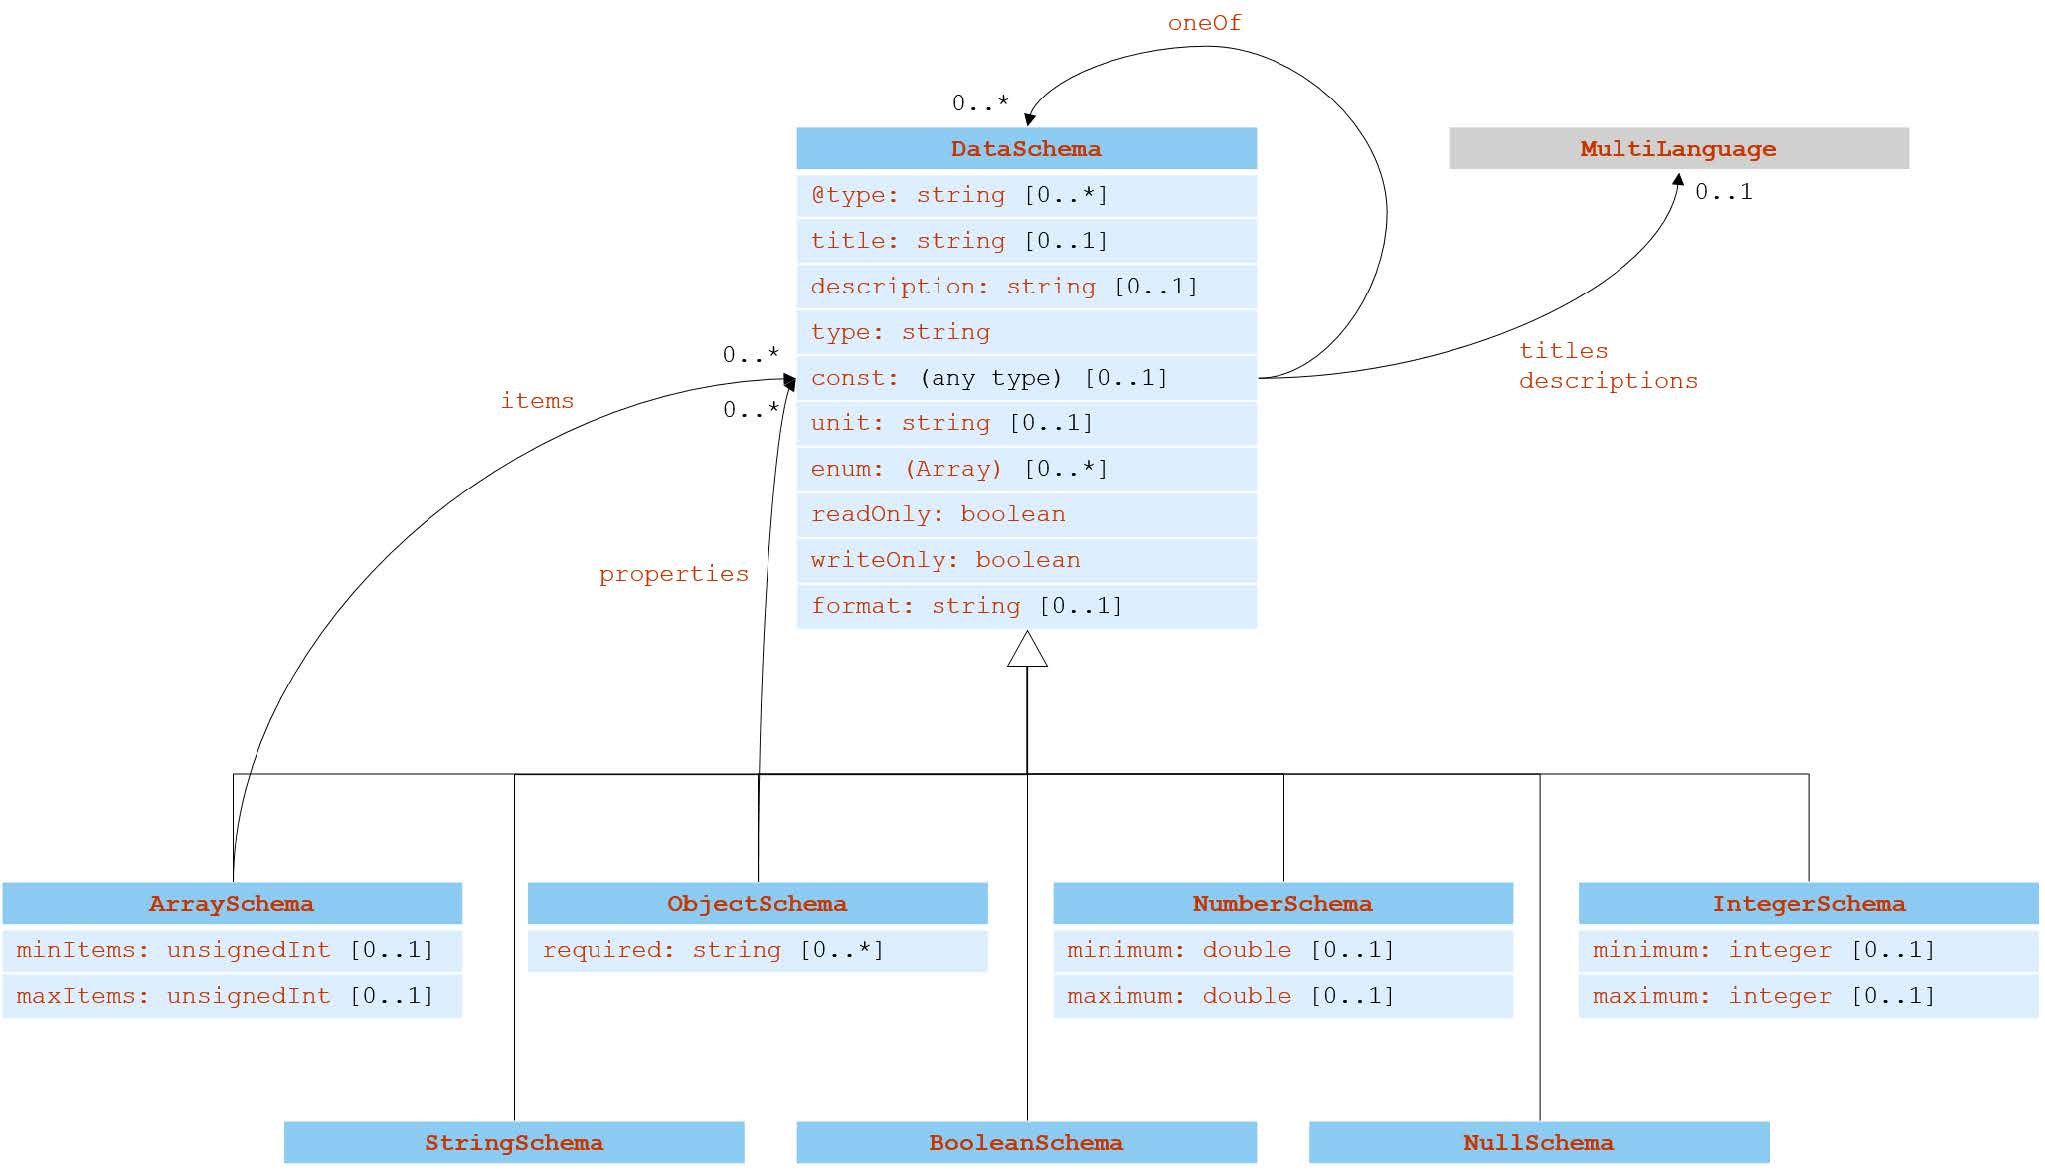
\includegraphics[width=\textwidth]{td-data-schema-vocabulary.jpg}
  \caption{\glsxtrshort{td} Datenschemavokabular}\label{fig:td_data_schema_vocabulary}
\end{figure}

\subsubsection{Sicherheitsvokabular}

Das Sicherheitsvokabular definiert Sicherheitsmechanismen und dessen Konfigurationen.

\begin{figure}[H]
  \centering
  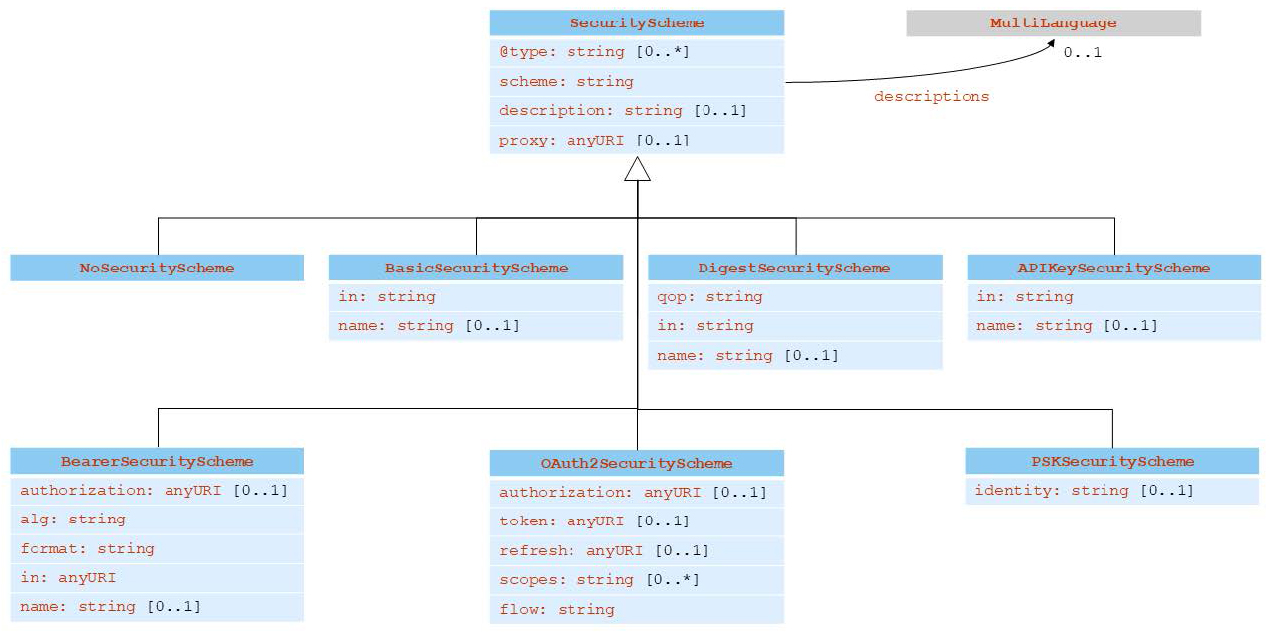
\includegraphics[width=\textwidth]{td-security-vocabulary.jpg}
  \caption{\glsxtrshort{td} Sicherheitsvokabular}\label{fig:td_security_vocabulary}
\end{figure}

Ein \lstinline{SecurityScheme} beinhaltet dabei grundsätzlich einen Bezeichner für das jeweilige Sicherheitsschema und möglicherweise Beschriftungen oder einen \glsxtrshort{uri}, auf die das Sicherheitsschema einen möglichen Zugriff definiert -- wenn es nicht um den aktuellen \glsxtrshort{uri} geht. Der Schemabezeichner wird dabei als Diskriminator für die einzelnen Sicherheitsschemata verwendet. Dabei sind je nach Sicherheitsschema weitere Objektattribute erforderlich oder möglich.

\subsubsection{Hypermediakontrollvokabular}

Das Hypermediakontrollvokabular definiert die Hauptbestandteile von Kommunikation über \gls{rest} mit Verweisen und Formularen.

\begin{figure}[H]
  \centering
  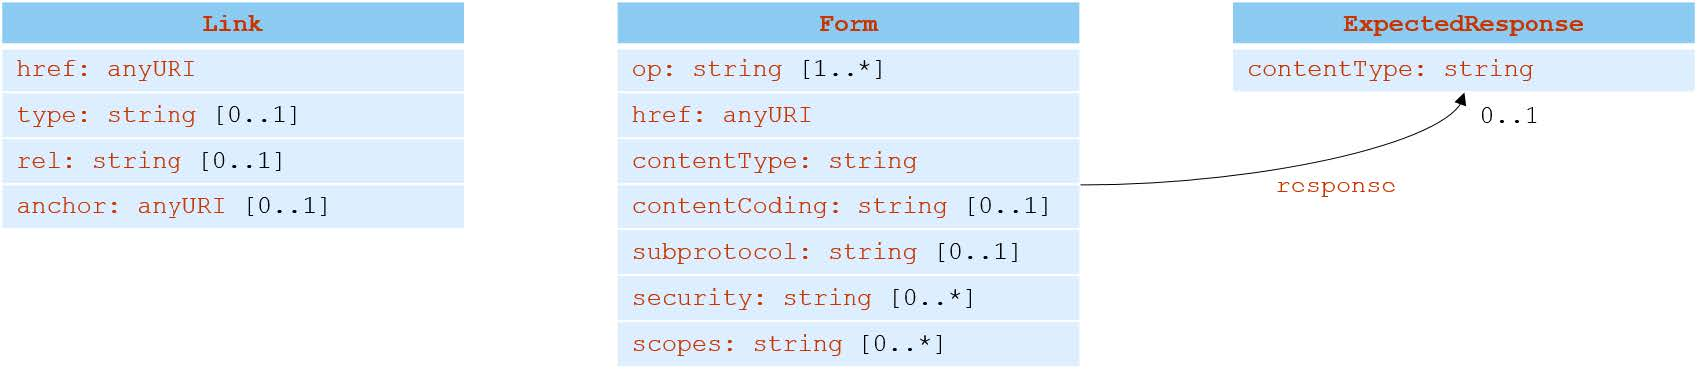
\includegraphics[width=\textwidth]{td-hypermedia-controls-vocabulary.jpg}
  \caption{\glsxtrshort{td} Hypermediakontrollvokabular}\label{fig:td_hypermedia_controls_vocabulary}
\end{figure}

\lstinline{Link}s funktionieren dabei sehr ähnlich zu Ankerelementen in \gls{html}. Sie bestehen hauptsächlich aus einem \gls{iri} und können durch den Medientyp des Ergebnisses, eine Relationsbeschreibung und einen Linkkontext erweitert werden.

\lstinline{Form}s werden an vielen Stellen verwendet. Sie bestehen hauptsächlich aus einem Bezeichner für die Operation(en), die durchgeführt werden soll(en), sowie aus einem \gls{iri}, der beschreibt, wohin das Formular geschickt werden soll. Es können noch weitere Werte ergänzt werden, wie die Art und Codierung des Inhalts, das verwendete Subprotokoll, Sicherheitsaspekte oder die Art der Antwort.

\subsection{Discovery}\label{subsec:wotdiscovery}

Die \glsxtrshort{wt}-Discovery beschreibt einen Prozess, mit dem eine \glsxtrfull{td} gefunden werden kann.
Dabei soll die Verbreitung in einer Vielzahl von Anwendungsfällen unterstützen werden, wie Beispielsweise in lokalen und öffentlichen Netzwerken.
Der Prozess muss dabei mit bestehenden Discovery-Mechanismen funktionieren, sicher sein und private Informationen schützen.
Es muss ebenfalls in der Lage sein, Aktualisierungen von \glspl{td} effizient zu handhaben.

\begin{figure}[H]
    \centering
    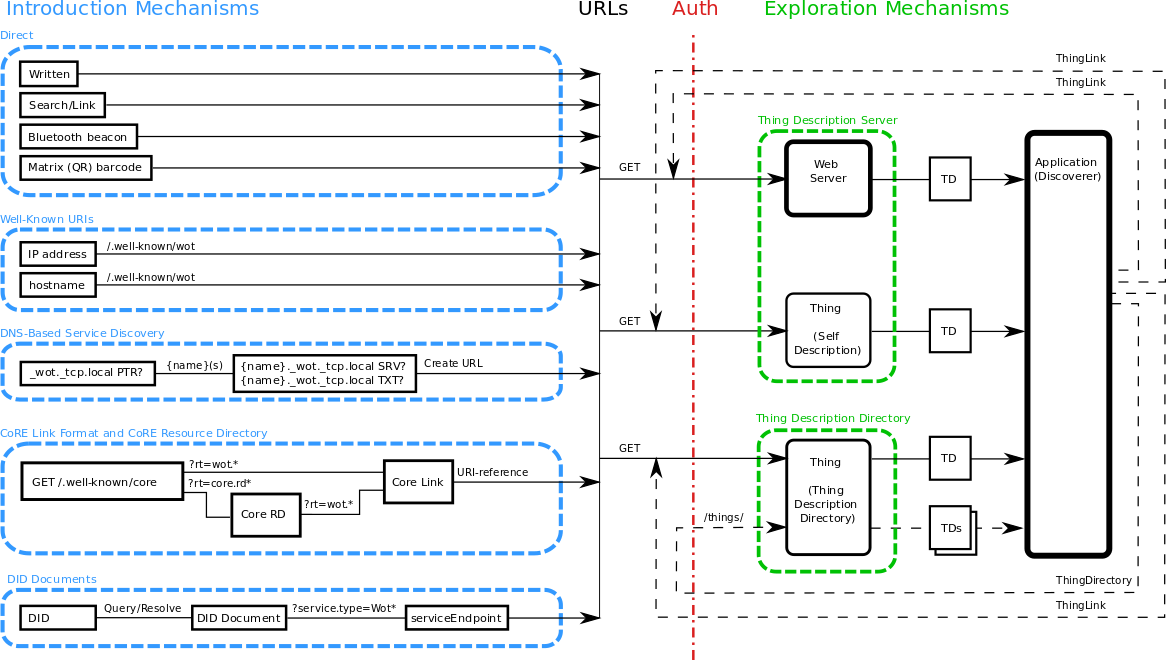
\includegraphics[width=16cm]{discovery-overview.png}
    \caption{Discovery-Architektur}\label{fig:discovery_overview}
\end{figure}

Der \gls{sd} Prozess ist dabei in zwei Phasen unterteilt, die Einführungs- und die Erkundungsphase.
Die Einführungsphase nutzt bestehende Erkundungsmechanismen, um ein oder mehrere \glspl{url} zu erzeugen.
Diese \glspl{url} enthalten selbst keine Metadaten und verweisen auf Erkundungsdienste.
Erst diese Erkundungsdienste stellen dann Metadaten in Form von \gls{td}[s] und \glspl{tdd} bereit.
Dabei gibt es zwei Arten von Erkundungsdiensten:

\begin{itemize}
    \item Ein Dienst, der sich um die Verteilung einer einzelnen \gls{td} kümmert, wie z.\,B.\ ein einfacher Webservice.
    \item Ein Dienst für das Durchsuchen eines \gls{tdd}[s], worin sich mehrere \gls{td}[s] befinden.
\end{itemize}

Der Discovery-Prozess verwendet eine zweistufige Architektur.
Im ersten Schritt generieren die Einführungsmechanismen \glspl{url}, die dann in der Erkundungsphase referenziert und mit Metadaten verknüpft werden.
Die Einführung kann durch jeden Mechanismus durchgeführt werden, der eine \gls{url} liefern kann.
Der Einführungsmechanismus kann dabei auch mehrere \glspl{url} liefern, die in der Erkundungsphase in mehreren \glspl{td} resultiert.
Eine \gls{url}, die von einem Einführungsmechanismus zur Verfügung gestellt wird, zeigt dabei immer auf einen Endpunkt eines Erkundungsmechanismus, der eine \gls{td} liefert.
Dies ist im einfachsten fall eine gewöhnliche Ressource, die von einem Webserver bereitgestellt wird und eine \gls{td} zurückgibt.
Im Sonderfall gibt es noch eine selbst beschreibende \gls{url} für ein \gls{thing}, was seine eigene \gls{td} liefert.

Jeder Client, der eine einzelne \gls{td} mit einer einzelnen \gls{url} abrufen kann, unterstützt \glsxtrshort{wot}-Discovery.
Sie muss dabei aber gewisse Anforderungen erfüllen, wie z.\,B.\ dass mindestens ein Einführungsmechanismus vorhanden sein muss
oder das mehrere Aufrufe desselben Einführungsmechanismus möglich sind.
Diese Anforderungen sorgen dafür, dass genau definiert ist, wie sich die \gls{td} in verschiedenen Szenarien verhalten soll.
Es können verschiedene Einführungsmechanismen verwendet werden, wie z.\,B.\ die direkte Variante über eine \gls{url}, eine Variante mit DNS-basierter Service-Discovery, oder eine Variante mithilfe von \gls{core}.
Das Ergebnis ist aber immer eine \gls{url} eines Erkundungsmechanismus, welcher die Metadaten einer \gls{td} beinhaltet.

Im Erkundungsprozess werden \glspl{td} mithilfe von zwei Mechanismen über einen Server zur Verfügung gestellt.
Jeder Webdienst, der über eine \gls{url} referenziert werden kann und eine \gls{td} zurückliefert, kann als Erkundungsmechanismus verwendet werden und wird als \glsxtrshort{td}-Server bezeichnet.
Ein \glsxtrshort{td}-Server muss dabei nicht zwangsläufig ein \gls{thing} sein, sondern kann auch über ein einfachen Webserver implementiert werden.
\glsxtrshort{td}-Server können auch zur Selbstbeschreibung verwendet werden. Für die Selbstbeschreibung hostet ein \gls{thing} seine eigene \gls{td} und stellt sie zur Verfügung.
Neben \glsxtrshort{td}-Servern gib es noch die bereits erwähnten \glspl{tdd}, worin sich keine oder mehrere \gls{td}[s] befinden und verwaltet werden können.
Für jede \gls{td} enthält das \gls{tdd} zusätzliche Metadaten für Buchführungs- und Suchzwecke.

\subsection{Sicherheit \& Datenschutz}\label{sec:wotsecurityprivacy}

Die Sicherheit eines \glsxtrshort{wot}-Systems kann sich auf die Sicherheit der \gls{td} selbst, oder auf die Sicherheit des \gls{thing}[s] beziehen.
Das \gls{wot} führt keine neuen Sicherheitsmechanismen ein. Es wird lediglich garantiert, dass bestehende Funktionalität und Sicherheit der Systeme beibehalten wird.
Hierbei werden verschiedene Anforderungen gestellt. Bei der Offenlegung einer \gls{td} sollte es z.\,B.\ möglich sein, bewährte Verfahren für die Sicherheit und Integrität anzuwenden.
Eine \gls{td} sollte zudem den tatsächlichen Sicherheitsstatus des von ihr beschriebenen Geräts genau wiedergeben.
Das \gls{wot} kann potenziell auf viele Protokolle angewendet werden. Für die Begrenzung des Umfangs wird sich aber hauptsächlich auf HTTP(S), CoAP(S) und MQTT(S) konzentriert.
Das \gls{wot} stellt zudem ein Framework bereit, welches eine Reihe möglicher Bedrohungen und Sicherheitsziele auflistet, die ein Anwender berücksichtigen sollten.
Des Weiteren werden Sicherheitspraktiken für die Gestaltung einer \gls{td} beschrieben, sowie ein Beispiel für eine sichere Konfiguration vorgeführt.

Mehrere Bedrohungen können die Privatsphäre von \glsxtrshort{wot}-Betreibern beeinträchtigen. Ein Betreiber kann hier z.\,B.\ eine Person sein, die ein Smart-Home besitzt,
oder eine Firma, die mehrere \glsxtrshort{wot}-\glspl{thing} in einer Fabrik betreibt.
Eine \gls{td} kann z.\,B.\ datenschutzrelevante Informationen preisgeben, wie die detaillierte Konfiguration eines einzelnen \gls{thing}[s].
Es können ebenfalls datenschutzrelevante Informationen durch Beobachtung der Kommunikation zwischen einem WoT-Endpunkt (Client, Server oder Gerät) und einer \gls{tdd} ermittelt werden.
Abhängig von der Netzwerktopologie können \glsxtrshort{wot}-Systeme Betreiberdaten zwischen dem \glsxtrshort{wot}-Konsumenten und dem \glsxtrshort{wot}-\gls{thing} über viele Zwischenknoten übertragen werden.
Wenn diese Knoten auf die Betreiberdaten zugreifen oder sie verarbeiten, kann es dazu kommen, dass ungewollt Informationen preisgeben werden.
Zusätzlich zu den oben beschriebenen Maßnahmen ist es wichtig, die Betreiber über die gesammelten Daten zu informieren und ihnen die Möglichkeit zu geben, den Grad dieser Offenlegung zu kontrollieren.


\section{Diskussion}\label{sec:discussion}

Aus der gesammelten Recherche geht hervor, dass sich die vorgestellten \glspl{sd} nicht optimal eignen, um als \gls{sd} einer Schnittstelle zu dienen, über die Städte gesammelte Daten öffentlich zugänglich machen können.
Bei allen Varianten besteht das Hauptproblem dabei darin, dass keinerlei Standardisierung vorhanden ist. Das bedeutet nicht, dass man diese Ansätze nicht dennoch weiter verfolgen könnte, aber es empfiehlt sich, stattdessen mit den Standards des \gls{wot} zu arbeiten.

Dabei lässt sich als Erstes festhalten, dass auch die Standards des \gls{w3c} \autocite{w3c.wot.architecture.20200408, w3c.wot.td.20200623, w3c.wot.bt.20200130, w3c.wot.scriptingapi.20201124, w3c.wot.discovery.20210602, w3c.wot.spg.20191106} für das \gls{wot} noch nicht vollständig erstellt wurden. Das hat zur Folge, dass einige Aspekte zum aktuellen Zeitpunkt noch unklar sind und sich Hintergründe der Spezifikationen nicht immer nachvollziehen lassen. Obwohl es nicht immer ratsam ist, sich auf unfertige Arbeiten zu beziehen, kann davon ausgegangen werden, dass diese Arbeiten später die Grundlage für noch fehlende Standards bilden werden und daher als Grundlage genutzt werden können.

Die Spezifikationen decken zu diesem Zeitpunkt noch keine \glsxtrshort{qos}[-basierte] \gls{sd} ab. Unter anderem Informationen zur Verfügbarkeit und Aktualisierungsrate von Services können daher nicht direkt mit in Betracht genommen werden. An dieser Stelle haben wir weiterhin nach Möglichkeiten recherchiert, \gls{qos}[-Aspekte] zu beachten. Unter anderem wird in \citetitle{Sciullo.DeterministicIndustrialNetworkingWebOfThings.2020} \autocite{Sciullo.DeterministicIndustrialNetworkingWebOfThings.2020} ein erweitertes Vokabular für \glspl{td} vorgestellt, mit dem \gls{qos}[-Aspekte] definiert werden können.

Die Sicherheitsaspekte, die vom \gls{w3c} für das \gls{wot} beschrieben werden, müssen bei der Entwicklung der bereits erwähnten Schnittstelle nicht weiter in Betracht gezogen werden.
Bei Daten, die von Städten zur Verfügung gestellt werden, handelt es sich meist um Open-Data, wo die Daten ohnehin frei zugänglich sind. Da es sich zudem nicht um personenbezogene Daten handelt, muss auch der Datenschutz nicht weiter beachtet werden.

Ein Problem, das teilweise bestehen bleibt, ist die Ontologie bei der Suche nach Services. Mit den beschriebenen Ansätzen ist es möglich, diese bei der \gls{sd} in Betracht zu ziehen, aber es gibt keine allgemeingültigen Ontologien, die dafür verwendet werden können. Es ist daher nötig, eine eigene Ontologie zu erstellen.

\section{Fazit}\label{sec:conclusion}

Die Recherche im Rahmen eines Ansatzes für eine Open-Data-Schnittstelle in Smart Cities hat gezeigt, dass die \gls{wot} vom \gls{w3c} einen guten Ansatz bieten, um nach diesem Schema eine entsprechende Schnittstelle zu implementieren. Die Standards des \gls{w3c} bieten Standardisierungen, die z.\,B.\ das Beschreiben von Sensoren als auch die \gls{sd} abdecken. Zudem handelt es sich im Vergleich zu den untersuchten \gls{sd}-Aufbauten um aktuelle und sehr umfangreiche Beschreibungen des Standards. An einigen Stellen ist der Standard jedoch noch nicht vollständig ausgearbeitet.

Die Nutzung der diskutierten \gls{sd} aus den entsprechenden Papern hat sich als nicht sinnvoll herausgestellt, da diese oft für spezifische Anwendungsfälle entwickelt worden sind und somit keine Standardisierung vorhanden ist. Daher wird empfohlen, sich bei der Implementierung einer Schnittstelle an dem \glsxtrshort{wot}-Standard zu orientieren, der zusätzlich den Vorteil mitbringt, dass er nicht nur die \gls{sd} beschreibt.


\newpage
\phantomsection{}
\addcontentsline{toc}{section}{\listfigurename}
\listoffigures

%\phantomsection{}
%\addcontentsline{toc}{section}{\listtablename}
%\listoftables

\printglossaries{}

\printbibliography[heading=bibintoc]

\end{document}
